\documentclass[11pt]{article}
\usepackage[croatian]{babel}
\usepackage{hyperref}
\usepackage{graphicx}

\hypersetup{
    colorlinks=true,
    linkcolor=black,
    urlcolor=black,
    pdftitle={Overleaf Example},
    pdfpagemode=FullScreen,
}

\topmargin -.5in
\textheight 9in
\oddsidemargin -.25in
\evensidemargin -.25in
\textwidth 7in

\begin{document}

\author{Matija Halavanja, Marin Hanić}
\title{Šah - Multimedijski sustavi}
\maketitle
\tableofcontents

\section{Opis programa}
Za projekt iz kolegija Multimedijski sustavi odlučili smo napraviti šah u programskom jeziku Javascript koristeći p5.js.
Odlučili smo se za p5.js umjesto Processinga jer smo htjeli u isto vrijeme istražiti taj library i napraviti projekt koji
bi bio dostupan na webu. Šah je igra za dva igrača s pravilima koji su poznati većini ljudi pa ih sada nećemo ovdje objašnjavati.
Figure se pomiču tako da kliknemo i povućemo na željeno polje. Ako figura po pravilima šaha ne može doći na to polje, vraća se na
početno mjesto i isti igrač je i dalje na potezu. Projekt je hostan na \url{https://mhalavanja.github.io/}, ali "službeno" kod aplikacije je
na \url{https://github.com/MarinHanic0/MMS-chess}. Kako aplikacija izgleda možemo vidjeti na sljedećoj \hyperref[igra]{slici 1}.

\begin{figure}[ht!]
    \centering
    \caption{Izgled aplikacije}
    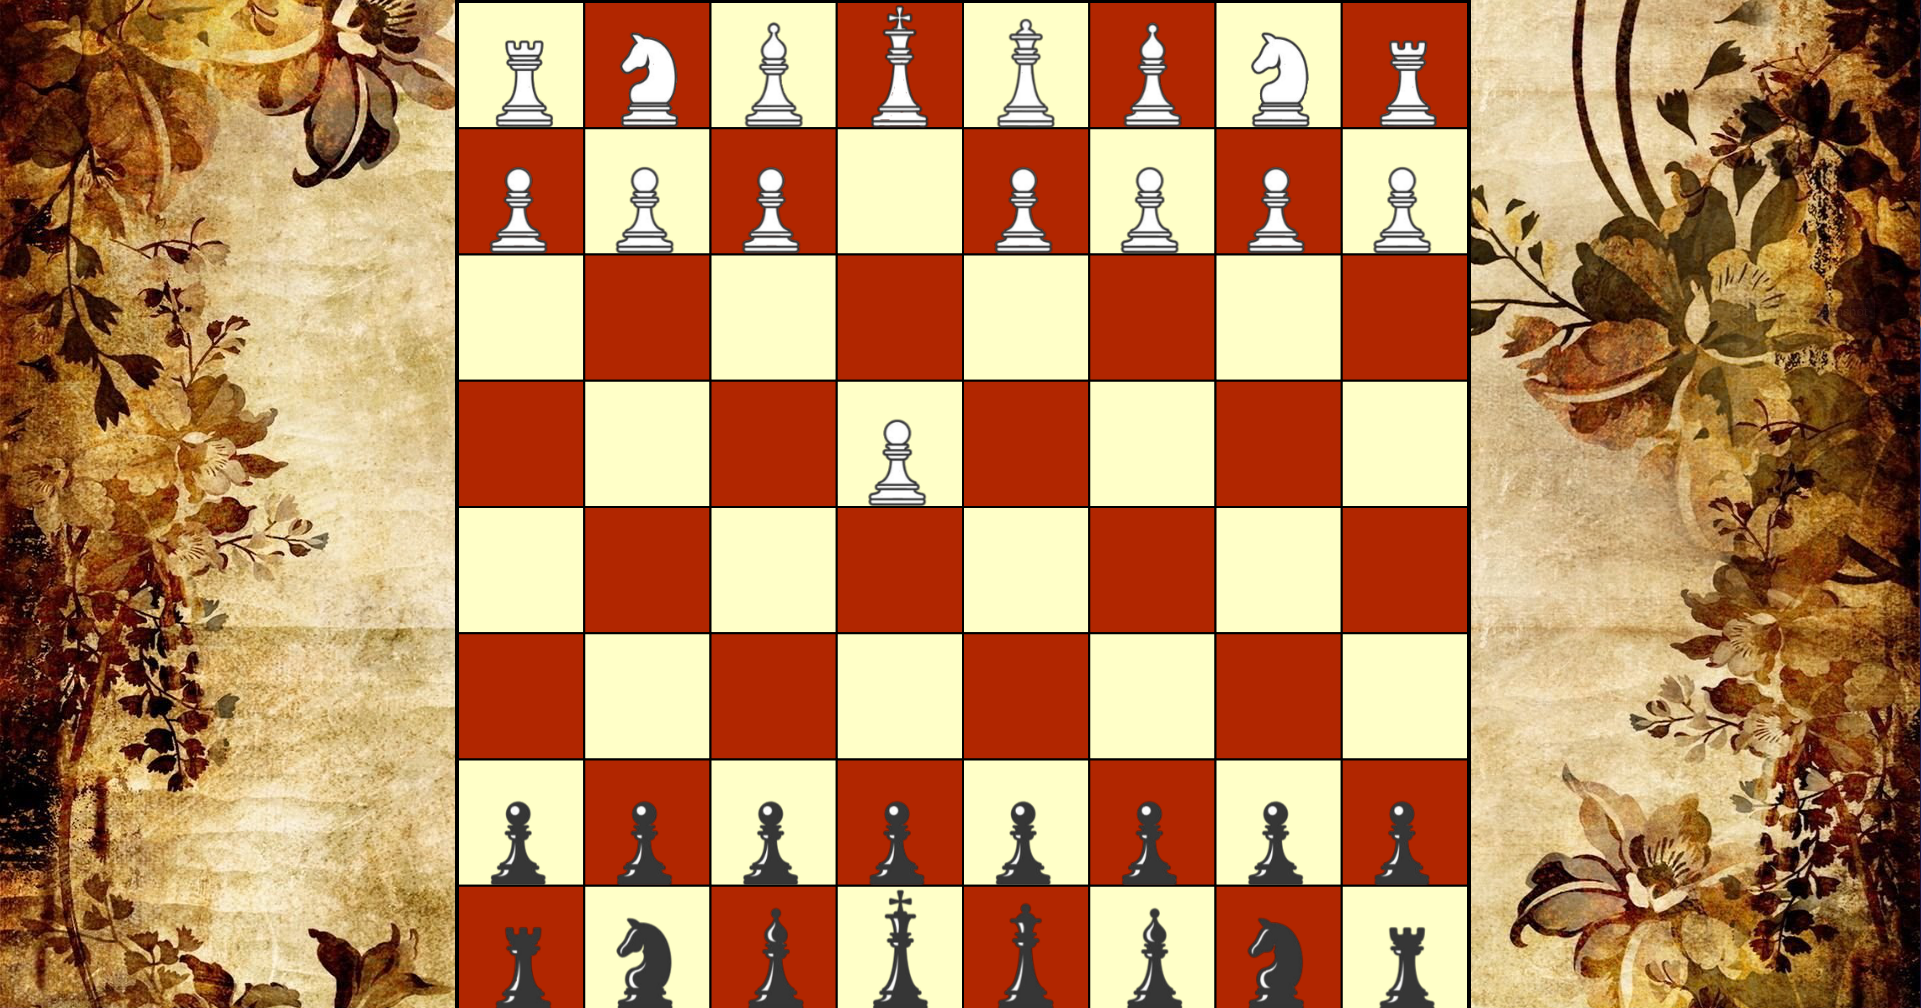
\includegraphics[scale=0.3]{igra.png}
    \label{igra}
\end{figure}

\section{Dizajn programa}
Program se dijeli na dva dijela. Prvi dio je usko vezan uz p5.js te obuhvaća sve što korisnik aplikacije vidi i kako
interagira s aplikacijom. Većina tog dijela aplikacije se nalazi unutar \textit{sketch.js} datoteke. Drugi dio aplikacije je logički prikaz
svih događaja koji su posljedica prikaza i interakcije korisnika s aplikacijom. Između osdtalog, to znači da moramo na početku 
postaviti sve figure na početne pozicije, validirati je li određeni potez moguć ili ne, registrirati kraj partije te
registrirati dolazak pješaka na zadnji red ploče. Svaka figura je implementirana u zasebnoj klasi koja se nalazi u zasebnoj datoteci.
Svaka klasa figure extenda generičku klasu \textit{Piece} u kojoj se nalaze neke zajedničke funkcije i svojstva. Također, postoji posebna
klasa \textit{Board} koja predstavlja ploču i objedinjuje logiku pomicanja figura po šahovskim pravilima koja se za svaki potez moraju
provjeravati. Takva klasa mora postojati radi hrpe šahovskih pravila npr. ako je kralj u šahu, igrač mora napraviti neki potez tako da mu ne
bude šah nakon tog poteza. Radi takvih pravila trebamo stalno pratiti koja polja svaki igrač napada sa svojim figurama. Da bi to postigli,
za svaku figuru moramo imati funkciju koja nam ovisno o trenutnom polju na kojem se nalazi i ostalim figurama na ploči, vraća na koja polja
se ta figura može pomaknuti. Ta ista polja su i također polja koja ta figura napada. Jedina iznimka tomu je en passant koji je morao onda posebno
biti implementiran.Svaka figura još implementira funkcije potrebne za njeno pravilno pomicanje i smještena je u vlastitoj datoteci i vlastitoj klasi.
Te klase nećemo posebno spominjati ovdje, nego ćemo se fokusirati na prethodno spomenute tri datoteke odnosno klase.

\subsection{sketch.js}
Datoteka sadrži varijable potrebne za pravilno iscrtavanje ploče i figura te se brine o tome što se događa na pritisak 
tipke miša i njeno otpuštanje.\\
Funkcija \textit{setup} kreira instancu klase \textit{Board} i priprema canvas.\\
Funkcija \textit{draw} iscrtava ploču i figure na njoj, ovisno o tome je li figura spuštena ili podignuta.\\
Funkcije \textit{mousePressed} i \textit{mouseReleased} služe za prepoznavanje podizanja i spuštanja figure na polje. Moraju paziti da
se miš nalazi unutar okvira ploče i odrediti o kojem polju se točno radi.\\
Funkcija \textit{choosePiece} sadrži dio logike potreban kod promocije pijuna u figuru.\\

\subsection{Board}
Klasa \textit{Board} je najveća klasa u projektu. To je zato što se u njoj provjeravaju sva pravila šaha pri pomicanju figura koja
uključuju interoperabilnost figura. Također sadrži puno jednostavnih, pomoćnih funkcija od po svega par linija koje nećemo spominjati tu.\\
Funkcija \textit{getMovingPiece} za dano polje vraća referencu na figuru koja se nalzi na tome polju.\\
Funkcija \textit{showMovingPiece} se brine da se slika figure pokazuje ispravno pri pomicanju figure mišem.\\
Funkcija \textit{startPieces} inicijalizira i vraća figure za danog igrača.\\
Funkcija \textit{makeMove} pomiče odabranu figuru na dano polje. Iz ove se funkcije onda poziva večina logike u aplikaciji jer se pritom svakog
poteza mora provjeriti da je potez legalan po pravilima šaha.\\  
Funkcija \textit{isGameOver} poziva pomočne funkcije i provjerava je li igra gotova.
Funkcija \textit{isTherePossibleMove} se koristi kod provjere pata.\\
Funkcija \textit{canPreventCheck} se koristi kod provjere mata jer ako igrač ne može nikako spriječiti šah, zapravo je u matu.\\
Funkcija \textit{checkPawnToPieceChange} je prvi dio logike provjere je li pješak došao do zadnjeg reda za promociju. \\
Funkcija \textit{isCausingSelfCheck} provjerava da pomicanjem dane figure igrač ne prouzročuje šah sam sebi. Primjer toga je kada je
npr. skakač između svog kralja i protivničkog topa pa se ne smije pomaknuti.\\
Funkcija \textit{setCheck} postavlja svojstvo \textit{inCheck} objekta klase \textit{King} na true ako je protivnik svojim zadnjim potezom
dao šah.\\
Funkcija \textit{show} se poziva u \textit{sketch.js} u funkciji \textit{draw}, a služi za grafički prikaz ploče i svih figura. 

\subsection{Piece}
Ova klasa obuhvaća svojstva i funkcije koje svaka druga klasa koja prestavlja figuru extenda.
Funkcija \textit{setSquare} zadužena je za pravilni logički i grafički prikaz figure na dano polje pri njenom pomicanju. 
Funkcije \textit{show} i \textit{moveImage} se brinu za pravilan prikaz slika figura na ploči, ovisno o polju na kojem se nalaze ili poziciji miša.
Funkcija \textit{isPlayableSquare} provjerava je li figura može biti odigrana na dano polje, ovisno o tome je li polje prazno i kojem igraču pripada.
Funkcija \textit{checkCapture} provjerava je li pri pomicanju figure neka protivnička figura pojedena.
Funkcija \textit{isDouleCheck} provjerava je li kralj danog igrača u duplom šahu. To je potrebno provjeravati jer u toj situaciji nije dovoljno pojesti
figuru koja zadaje šah, nego jedini način da kralj ne bude u šahu je da se pomakne.

\section{Poboljšanja}
Neka moguća poboljšanja su:
\begin{itemize}
    \item Uvođenje vremenske kontrole za svakog igrača po partiji
    \item Uvođenje izbora vremenske kontrole, npr 3 min po igraču plus 2 sekunde po potezu, 5 min po igraču
    \item Zapisivanje odigranih poteza
    \item Mogućnost lokalnog spremanja odigranih poteza u datoteku
    \item Mogućnost izbora izgleda figura i ploče
    \item Dodavanje opcije okretanja ploče tako da figure igrača koji je na potezu budu dolje radi lakšeg pregleda ploče
    \item Dodati pripadne oznake A-H i 1-8 za stupce odnosno redke na ploči
    \item Dodavanje različitih verzija šaha
    \item Dodati glazbu
    \item Označiti polja na koja podignuta figura može odigrati potez
\end{itemize} 

\section{Literatura}
\begin{itemize}
    \item https://p5js.org/
    \item https://developer.mozilla.org/en-US/docs/Web/JavaScript
\end{itemize}
\end{document}